% TODO standardize naming: marking vs mark insertion, marks vs error marks vs markings
% TODO uniform style for referencing rules

\section{The Marked Lambda Calculus}
\label{sec:calculus}

Programmers often work with program states that are syntactically well-formed but not well-typed.
\Cref{fig:calculus-examples} shows common type errors as they appear in the Hazel programming
environment. For example, a simple error that may occur is the use of an unbound variable. As in
\cref{fig:calculus-examples-unbound}, editor services indicate the usage of unbound $y$ is invalid
by highlighting it in red.

\begin{figure}[htbp]
  \begin{tabular}[b]{cc}
    \begin{subfigure}[b]{0.3\columnwidth}
      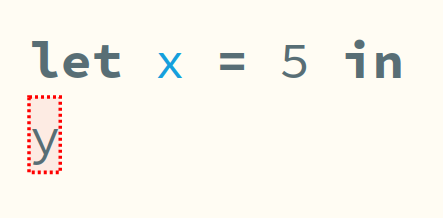
\includegraphics[width=\columnwidth]{images/haz3l-unbound-variable.png}
      \caption{Unbound variable error.}
      \label{fig:calculus-examples-unbound}
    \end{subfigure}
    &
    \begin{subfigure}[b]{0.3\columnwidth}
      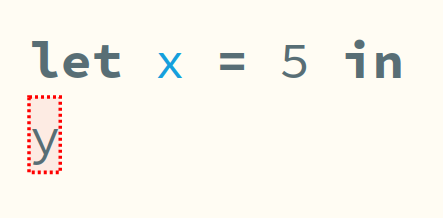
\includegraphics[width=\columnwidth]{images/haz3l-unbound-variable.png}
      \caption{Inconsistent types error.}
      \label{fig:calculus-examples-inconsistent-types}
    \end{subfigure} \\
    \begin{subfigure}[b]{0.3\columnwidth}
      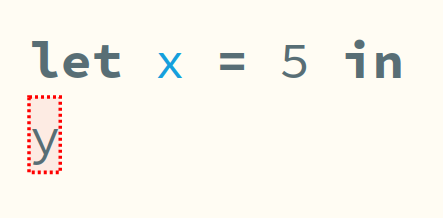
\includegraphics[width=\columnwidth]{images/haz3l-unbound-variable.png}
      \caption{Application of a non-lambda.}
      \label{fig:calculus-examples-app-non-lambda}
    \end{subfigure}
    &
    \begin{subfigure}[b]{0.3\columnwidth}
      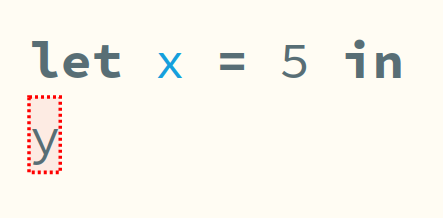
\includegraphics[width=\columnwidth]{images/haz3l-unbound-variable.png}
      \caption{Inconsistent branches error.}
      \label{fig:calculus-examples-inconsistent-branches}
    \end{subfigure}
  \end{tabular}
  %
  \caption{Examples of common type errors.}
  \label{fig:calculus-examples}
\end{figure}


Sometimes, the type an expression \emph{should} be is known. Consider
\cref{fig:calculus-examples-inconsistent-types}, in which it is expected that both operands of the
$+$ operator are numbers. Since $\textsf{true}$ is not a number, a type error arises, and Hazel
indicates a mismatch between the expected and actual types of the operand. The application in
\cref{fig:calculus-examples-app-non-lambda} of a non-lambda leads to a similar kind of error. In
this case, however, the expectation is not a singular type, but any member of a family of function
types. \Cref{fig:calculus-examples-inconsistent-branches} presents an error of inconsistent
branches: the branches of the if-else expression are of different types. Hazel opts to highlight the
entire expression in such a situation, while other tools may choose one branch to be ``correct'' and
``blame'' the type mismatch error on the other.

% TODO elaborate on this part

Unfortunately, formal typing semantics usually only give meaning to well-typed programs, leaving
such ill-typed ones meaningless. This is insufficient for editor services and language servers,
which must provide users feedback on where and why a program is ill-typed. Moreover, they must
continue providing semantic services even when an error is encountered. Indeed, similarly to
error-recovering parsers, real-world type checkers must robustly recover from type errors.
Traditionally, this has been performed in an \emph{ad hoc} manner [citations?], with different
languages and tools adopting varying approaches in the localization, reportage, and recovery of
errors.

% TODO examples of this ad hoc stuff

The key contribution of this section is the \emph{marked lambda calculus}, a formal calculus for
type error localization in bidirectional systems. Namely, the calculus provides a judgmental
framework with a unified theory for the design of typing semantics that support ill-typed programs.
\Cref{sec:calculus-calculus} describes its form and metatheory by example on a small gradually typed
lambda calculus, extending it with binary product types in \cref{sec:calculus-products}. All rules
and theorems may be found in the supplementary appendix, alongside a complete mechanization in the
Agda proof assistant, which is discussed briefly in \cref{sec:calculus-agda}. With products, we then
consider how error localization is complicated by patterned let expressions in
\cref{sec:calculus-let}. Finally, \cref{sec:calculus-poly} explores how the system might be extended
to more complex typing features, such as System F-style polymorphism.

% TODO not really sure when to start talking about bidirectional typing

% \emph{Bidirectional typing} combines type checking, which determines if a program satisfies a given
% type, and type synthesis, which generates a type from the program. This gives a simple algorithmic
% system in which type information is recursively propagated through terms and allows for local type
% inference.

% TODO talk about idea that bidirectional typing makes error localization easy? i.e. why choose
% bidirectional?

\subsection{The Calculus}
\label{sec:calculus-calculus}

% TODO outline the structure of this section at the beginning
% TODO make it clear unmarked/marked languages share same types

We now formally introduce the marked lambda calculus through its application to a gradually typed
lambda calculus extended with numbers and booleans. Consider the syntax for such a language, given
as $\EMName$ in \cref{fig:calculus-syntax}. The base types $\TNum$ and $\TBool$ classify number and
boolean expressions. The number literal corresponding to the mathematical number $n$ is given by
$\ENumMV$, and there is a single addition operation on numeric expressions. $\ETrue$ and $\EFalse$
correspond to the boolean values $\textsf{true}$ and $\textsf{false}$, respectively, and
$\EIf{\EMV_1}{\EMV_2}{\EMV_3}$ gives a conditional structure. In addition to these forms,
$\TUnknown$ is the unknown type from gradual type theory. $\EEHole$ denotes an \emph{expression
hole}, which are used to model syntactically incomplete programs---but are not critical within the
calculus.

\begin{figure}[htbp]
  \[\begin{array}{rrcl}
    \TMName  & \TMV  & \Coloneqq & \TUnknown \mid \TNum \mid \TBool \mid \TArrow{\TMV}{\TMV} \mid \TProd{\TMV}{\TMV} \\
    \EMName  & \EMV  & \Coloneqq & x \mid \ELam{x}{\TMV}{\EMV} \mid \EAp{\EMV}{\EMV} \mid \ELet{x}{\EMV}{\EMV}
                       \mid           \ENumMV \mid \EPlus{\EMV}{\EMV} \\
             &       & \mid         & \ETrue \mid \EFalse \mid \EIf{\EMV}{\EMV}{\EMV}
                       \mid           \EPair{\EMV}{\EMV}
                       \mid           \EProjL{\EMV} \mid \EProjR{\EMV}
                       \mid           \EEHole \\
    \ECMName & \ECMV & \Coloneqq & x \mid \ECLam{x}{\TMV}{\ECMV} \mid \ECAp{\ECMV}{\ECMV} \mid \ECLet{x}{\ECMV}{\ECMV}
                       \mid           \ECNumMV \mid \ECPlus{\ECMV}{\ECMV} \\
             &       & \mid         & \ECTrue \mid \ECFalse \mid \ECIf{\ECMV}{\ECMV}{\ECMV}
                       \mid           \ECPair{\ECMV}{\ECMV} \mid \ECProjL{\ECMV} \mid \ECProjR{\ECMV}
                       \mid           \ECEHole \\
             &       & \mid         & \ECUnbound{x} \mid \ECInconType{\ECMV} \mid \ECInconBr{\ECMV}{\ECMV}{\ECMV} \mid \ECInconAsc{\ECMV} \\
             &       & \mid         & \ECSynNonMatchedArrow{\ECMV} \mid \ECAnaNonMatchedArrow{\ECMV}
                       \mid           \ECSynNonMatchedProd{\ECMV} \mid \ECAnaNonMatchedProd{\ECMV}
  \end{array}\]
  \caption{Syntax of an extended gradually typed lambda calculus.}
  \label{fig:calculus-syntax}
\end{figure}

Types classify expressions by a \emph{bidirectional type system}, which employs two mutually defined
judgments. \emph{Type synthesis}, written $\ctxSynTypeU{\ctx}{\EMV}{\TMV}$, establishes that, under
the typing context $\ctx$, the expression $e$ synthesizes or infers the type $\TMV$. \emph{Type
analysis}, written $\ctxAnaTypeU{\ctx}{\EMV}{\TMV}$, states that the expression $\EMV$ may appear
where an expression of type $\TMV$ is expected. We may give these typing semantics traditionally,
without considering error localization and recovery.

The marked lambda calculus builds atop these typing semantics into a two-layer system:
%
\begin{itemize}
  \item The \textbf{unmarked language}, which is the original language. Expressions of this language
    are called \emph{unmarked expressions}, denoted by the metavariable $\EMV$.

  \item The \textbf{marked language}, which mirrors the structure of the unmarked language but is
    extended with explicit \emph{error marks}. We call expressions of this language to be
    \emph{marked expressions}, denoted $\ECMV$.
    % TODO more intuition for what marked expressions are?

  \item \textbf{Marking}, which \emph{marks}, i.e. type checks and localizes errors for, any unmarked
    expression into a marked expression, inserting error marks where appropriate.
\end{itemize}
%
In other words, we extend the ordinary typing semantics of a language with a secondary ``marked''
language and ``mark'' unmarked programs into marked ones. This corresponds to a type checking
process with error localization and recovery. The marked language may then serve as a foundation for
other semantic services. % such as THI.

% TODO more intuition

\Cref{fig:calculus-syntax} furthermore gives the syntax for marked expressions (as $\ECMName$),
which replicates all the forms of unmarked expressions. There are additionally several kinds of
\emph{error marks}, which represent the different type errors that may arise. Intuitively, they each
denote a different error message that might be shown in an editor or emitted by a compiler.
%
% \begin{itemize}
  % \item $\ECUnbound{x}$, the \emph{unbound variable mark}, indicates the use of an unbound variable
    % $x$, as in \cref{fig:calculus-examples-unbound}.
%
  % \item $\ECInconType{\ECMV}$, the \emph{inconsistent type mark}, indicates that the type of an
    % expression does not match an expected type.
%
  % \item $\ECInconBr{\ECMV_1}{\ECMV_2}{\ECMV_3}$, the \emph{inconsistent branches mark}, indicates
    % that the branches of a conditional have mismatched types.
%
  % \item $\ECLamInconAsc{x}{\TMV}{\ECMV}$, the \emph{inconsistent ascription mark}, indicates that
    % the type ascription $\TMV$ is mismatches with an expected type.
%
  % \item $\ECSynNonMatchedArrow{\ECMV}$
% \end{itemize}
%
Throughout the remainder of this section, as we formulate marking for the gradually typed lambda
calculus, we will motivate and give precise semantics for these error marks. Note that this is a
non-exhaustive list; depending on the syntactic forms and typing features found in the language,
other kinds of marks may be necessary. Indeed, in \cref{sec:calculus-poly}, we consider the kinds of
marks that may be required in an language with explicit polymorphism.

The marked language possesses its own typing semantics, also formulated bidirectionally. We write
$\ctxSynTypeM{\ctx}{\ECMV}{\TMV}$ for synthesis and $\ctxAnaTypeM{\ctx}{\ECMV}{\TMV}$ for analysis.
Finally, marking is bidirectional as well. The synthetic marking judgment
$\ctxSynFixedInto{\ctx}{\EMV}{\ECMV}{\TMV}$ establishes that, under the context $\Gamma$, the
unmarked expression $\EMV$ is ``marked into'' the marked expression $\ECMV$, which synthesizes type
$\TMV$. Analogously, the analytic marking judgment $\ctxAnaFixedInto{\ctx}{\EMV}{\ECMV}{\TMV}$
states that $\EMV$ is marked into $\ECMV$, which analyzes against $\TMV$.

How can we ensure that the marking procedure is correctly defined? There are two critical
metatheorems to keep in mind as we continue. The first is a \emph{totality} of marking:
%
\begin{theorem}[name=Marking Totality] \
  \label{thm:calculus-marking-totality}
  \begin{enumerate}
    \item For all $\ctx$ and $\EMV$, there exist $\ECMV$ and $\TMV$ such that
      $\ctxSynFixedInto{\ctx}{\EMV}{\ECMV}{\TMV}$.
    \item For all $\ctx$, $\EMV$, and $\TMV$, there exists $\ECMV$ such that
      $\ctxAnaFixedInto{\ctx}{\EMV}{\ECMV}{\TMV}$.
  \end{enumerate}
\end{theorem}
%
That is, we may mark \emph{any} syntactically well-formed program.

Furthermore, marking should preserve the syntactic structure of programs, modulo error marks. Thus,
we define a notion of \emph{mark erasure}, whose definition is given
\cref{fig:calculus-mark-erasure}, which converts marked expressions back into unmarked expression by
removing error marks. Then, \cref{thm:calculus-marking-well-formedness} provides a
\emph{well-formedness} criterion marking.
%
\begin{theorem}[name=Marking Well-Formedness] \
  \label{thm:calculus-marking-well-formedness}
  \begin{enumerate}
    \item If $\ctxSynFixedInto{\ctx}{\EMV}{\ECMV}{\TMV}$, then $\ctxSynTypeM{\ctx}{\ECMV}{\TMV}$ and
      $\erasesTo{\ECMV}{\EMV}$.
    \item If $\ctxAnaFixedInto{\ctx}{\EMV}{\ECMV}{\TMV}$, then $\ctxAnaTypeM{\ctx}{\ECMV}{\TMV}$ and
      $\erasesTo{\ECMV}{\EMV}$.
  \end{enumerate}
  % TODO split this into two theorems?
  % TODO not really sure how to intuitively describe the part about types matching up
\end{theorem}
%
In other words, marking and then erasing error marks from the result gives the original unmarked
expression. We also ensure that marking gives well-typed marked expressions; indeed, their types
should match the types synthesized or analyzed against in marking.
% TODO more intuition for this theorem

\begin{figure}[htbp]
  \newcommand{\erasesToRow}[2]{\erase{#1} & = & #2}
  \[\begin{array}{rcl}
    % \erasesToRow{\ECEHole}{\EEHole} \\
    \erasesToRow{x}{x} \\
    \erasesToRow{(\ECLam{x}{\TMV}{\ECMV})}{\ELam{x}{\TMV}{(\erase{\ECMV})}} \\
    \erasesToRow{(\ECAp{\ECMV_1}{\ECMV_2})}{\EAp{(\erase{\ECMV_1})}{(\erase{\ECMV_2})}} \\
    % \erasesToRow{(\ECLet{x}{\ECMV_1}{\ECMV_2})}{\ELet{x}{(\erase{\ECMV_1})}{(\erase{\ECMV_2})}} \\
    \erasesToRow{\ECNumMV}{\ENumMV} \\
    \erasesToRow{(\ECPlus{\ECMV_1}{\ECMV_2})}{\EPlus{(\erase{\ECMV_1})}{(\erase{\ECMV_2})}} \\
    \erasesToRow{\ECTrue}{\ETrue} \\
    \erasesToRow{\ECFalse}{\EFalse} \\
    \erasesToRow{(\ECIf{\ECMV_1}{\ECMV_2}{\ECMV_3})}{\EIf{(\erase{\ECMV_1})}{(\erase{\ECMV_2})}{(\erase{\ECMV_3})}} \\
    \erasesToRow{\ECUnbound{x}}{x} \\
    \erasesToRow{\ECInconType{\ECMV}}{\erase{\ECMV}} \\
    \erasesToRow{\ECInconBr{\ECMV_1}{\ECMV_2}{\ECMV_3}}{\EIf{(\erase{\ECMV_1})}{(\erase{\ECMV_2})}{(\erase{\ECMV_3})}} \\
  \end{array}\]
  %
  \caption{Mark erasure definition.}
  \label{fig:calculus-mark-erasure}
\end{figure}


In the remainder of this subsection, we consider the different type errors that may arise in the
unmarked language while keeping in mind these two theorems; in this way, the typing semantics of the
unmarked language guide the construction of the marking process.

\subsubsection{Numbers}
\label{sec:calculus-numbers}

To start, let us consider the simple case of numbers. Because of \emph{subsumption}, which we
discuss next, we need only define a synthesis rule for unmarked numbers, in which numbers synthesize
the type $\TNum$:
%
\begin{mathpar}
  \judgment{ }{
    \ctxSynTypeU{\ctx}{\ENumMV}{\TNum}
  }{USNum}
\end{mathpar}

How should numbers be marked? Quite straightforwardly, we simply give the same number as a marked
expression, synthesizing again $\TNum$. No type errors may occur in a single number, so we only need
the following rules for marking numbers and typing the results: 
%
\begin{mathpar}
  \judgment{
  }{
    \ctxSynFixedInto{\ctx}{\ENumMV}{\ECNumMV}{\TNum}
  }{MKSNum}

  \judgment{ }{
    \ctxSynTypeM{\ctx}{\ECNumMV}{\TNum}
  }{MSNum}
\end{mathpar}

For addition expressions, the type of both operands should be $\TNum$. To denote this in a
bidirectional system, the operands are analyzed against $\TNum$, giving the following typing rule
for unmarked addition expressions:
%
\begin{mathpar}
  \judgment{
    \ctxAnaTypeU{\ctx}{\EMV_1}{\TNum} \\
    \ctxAnaTypeU{\ctx}{\EMV_2}{\TNum}
  }{
    \ctxSynTypeU{\ctx}{\EPlus{\EMV_1}{\EMV_2}}{\TNum}
  }{USPlus}
\end{mathpar}

The marking rule mirrors \textsc{USPlus} closely. Since an expected type for each operand is known,
we shift the responsibility for any type errors to them. Hence, we recursively mark each operand in
analytic mode and rebuild the marked addition expression. The marked typing rule then mirrors
\textsc{USPlus} exactly.
%
\begin{mathpar}
  \judgment{
    \ctxAnaFixedInto{\ctx}{\EMV_1}{\ECMV_1}{\TNum} \\
    \ctxAnaFixedInto{\ctx}{\EMV_2}{\ECMV_2}{\TNum}
  }{
    \ctxSynFixedInto{\ctx}{\EPlus{\EMV_1}{\EMV_2}}{\ECPlus{\ECMV_1}{\ECMV_2}}{\TNum}
  }{MKSPlus}

  \judgment{
    \ctxAnaTypeM{\ctx}{\ECMV_1}{\TNum} \\
    \ctxAnaTypeM{\ctx}{\ECMV_2}{\TNum}
  }{
    \ctxSynTypeM{\ctx}{\ECPlus{\ECMV_1}{\ECMV_2}}{\TNum}
  }{MSPlus}
\end{mathpar}

\subsubsection{Subsumption}
\label{sec:calculus-subsumption}

Only synthetic rules were necessary for typing numbers and addition because of \emph{subsumption},
given below, which states that if an expression synthesizes a type, it may also be analyzed against
that type or any \emph{consistent} type.
\[%
  \judgment{
    \ctxSynTypeU{\ctx}{\EMV}{\TMV'} \\
    \consistent{\TMV}{\TMV'} \\
    \subsumable{\EMV}
  }{
    \ctxAnaTypeU{\ctx}{\EMV}{\TMV}
  }{UASubsume}
\]%
We rely on the notion of \emph{type consistency} from gradual type theory, which defines a reflexive
and symmetric (but not transitive) relation between types, writing $\consistent{\TMV_1}{\TMV_2}$ to
mean that $\TMV_1$ is consistent with $\TMV_2$. Defined in \cref{fig:calculus-consistency}, this
replaces the notion of \emph{type equality} to relate the unknown type to all other types.

\begin{figure}[htbp]
  \raggedright
  \judgbox{\ensuremath{\consistent{\TMV_1}{\TMV_2}}} $\TMV_1$ is consistent with $\TMV_2$
  %
  \begin{mathpar}
    \judgment{ }{
      \consistent{\TUnknown}{\TMV}
    }{TCUnknown1}

    \judgment{ }{
      \consistent{\TMV}{\TUnknown}
    }{TCUnknown2}

    \judgment{ }{
      \consistent{\TMV}{\TMV}
    }{TCRefl}

    \judgment{
      \consistent{\TMV_1}{\TMV_1'} \\
      \consistent{\TMV_2}{\TMV_2'} \\
    }{
      \consistent{\TArrow{\TMV_1}{\TMV_2}}{\TArrow{\TMV_1'}{\TMV_2'}}
    }{TCArr} \\
  \end{mathpar}
  %
  \caption{Type consistency.}
  \label{fig:calculus-consistency}
\end{figure}

Hence, when checking $\ENumMV$ against a known expected type, subsumption checks that the type is
consistent with $\TNum$, the type that $\ENumMV$ synthesizes. This succeeds for $\TUnknown$ and
$\TNum$.

We also restrict the usage of subsumption to ``subsumable'' syntactic forms, written
$\subsumable{\EMV}$. This judgment is defined on all syntactic forms except lambda abstractions and
conditionals, the only ones with explicit analysis rules. In other words, we restrict subsumption to
be the rule of ``last resort'', which is necessary to establish that marking and typing are
deterministic (discussed later in \cref{thm:calculus-marking-unicity}).

Now, to define analytic marking on forms without explicit analytic typing rules, we also need
subsumption rules for marking and marked expression typing. Note that we define a analogous notion
of ``subsumability'' for marked expressions, written $\subsumable{\ECMV}$.
%
\begin{mathpar}
  \judgment{
    \ctxSynFixedInto{\ctx}{\EMV}{\ECMV}{\TMV'} \\
    \consistent{\TMV}{\TMV'} \\
    \subsumable{\EMV}
  }{
    \ctxAnaFixedInto{\ctx}{\EMV}{\ECMV}{\TMV}
  }{MKASubsume}

  \judgment{
    \ctxSynTypeM{\ctx}{\ECMV}{\TMV'} \\
    \consistent{\TMV}{\TMV'} \\
    \subsumable{\ECMV}
  }{
    \ctxAnaTypeM{\ctx}{\ECMV}{\TMV}
  }{MASubsume}
\end{mathpar}

But what happens when the synthesized type of an expression is \emph{not} consistent with the
expected type, i.e. that the premise $\consistent{\TMV}{\TMV'}$ fails? Recalling the example of
\cref{fig:calculus-examples-inconsistent-types}, subsumption would be used to analyze $\ETrue$
against $\TNum$ in $\EPlus{\ETrue}{5}$, which fails since $\inconsistent{\TNum}{\TBool}$, i.e.
\textsc{UASubsume} does not apply, and traditional typing semantics would simply fail the type
checking process at this point. \textsc{MKASubsume} would also not be applicable, leaving marking
undefined in those cases.

% TODO use example more closely related to num here since we haven't talked about booleans yet?

To satisfy marking totality, such a possibility motivates an \emph{inconsistent type mark}
$\ECInconType{\ECMV}$, which states exactly that the synthesized type of $\ECMV$ is inconsistent
with the expected type. It is then accompanied by the following rules:
%
\begin{mathpar}
  \judgment{
    \ctxSynFixedInto{\ctx}{\EMV}{\ECMV}{\TMV'} \\
    \inconsistent{\TMV}{\TMV'} \\
    \subsumable{\EMV}
  }{
    \ctxAnaFixedInto{\ctx}{\EMV}{\ECInconType{\ECMV}}{\TMV}
  }{MKAInconsistentTypes}

  \judgment{
    \ctxSynTypeM{\ctx}{\ECMV}{\TMV'} \\
    \inconsistent{\TMV}{\TMV'} \\
    \subsumable{\ECMV}
  }{
    \ctxAnaTypeM{\ctx}{\ECInconType{\ECMV}}{\TMV}
  }{MAInconsistentTypes}
\end{mathpar}
%
Observe that the premises of \textsc{MKAInconsistentTypes} are identical to those of
\textsc{MKASubsume}, except that $\inconsistent{\TMV}{\TMV'}$. By marking an error, type-checking
may continue---instead of simply failing.

\subsubsection{Variables}
\label{sec:calculus-variables}

Let us now consider the case of variables. Typing in the unmarked language is standard, and because
of subsumption, only a synthetic rule is required:
\[%
  \judgment{
    \inCtx{\ctx}{x}{\TMV}
  }{
    \ctxSynTypeU{\ctx}{x}{\TMV}
  }{USVar}
\]%
That is, if $x$ is bound to a type in the typing context, it synthesizes that type.
Straightforwardly, marking converts an unmarked variable into the same variable via the following
rules:
%
\begin{mathpar}
  \judgment{
    \inCtx{\ctx}{x}{\TMV}
  }{
    \ctxSynFixedInto{\ctx}{x}{x}{\TMV}
  }{MKSVar}

  \judgment{
    \inCtx{\ctx}{x}{\TMV}
  }{
    \ctxSynTypeM{\ctx}{x}{\TMV}
  }{MSVar}
\end{mathpar}
% TODO more intuition on why this makes sense?

However, consider the case that a variable, such as $y$ in \cref{fig:calculus-examples-unbound}, is \emph{not}
bound. Again, \textsc{USVar} would not apply. A total marking should, however, report the error and
continue, motivating an \emph{unbound variable mark} $\ECUnbound{x}$ and the accompanying rules:
%
\begin{mathpar}
  \judgment{
    \notInCtx{\ctx}{x}
  }{
    \ctxSynFixedInto{\ctx}{x}{\ECUnbound{x}}{\TUnknown}
  }{MKSUnbound}

  \judgment{
    \notInCtx{\ctx}{x}
  }{
    \ctxSynTypeM{\ctx}{\ECUnbound{x}}{\TUnknown}
  }{MSUnbound}
\end{mathpar}
%
An unbound variable is marked as such, and since nothing may be said about their types, we
synthesize the unknown type. Similarly to the inconsistent type mark, this allows type checking to
proceed, with usage of the unbound variable permitted in any expression.
% TODO clarify/give intuition as to why this is correct

\subsubsection{Lambda Abstractions}
\label{sec:calculus-lambda-abstractions}

Unlike numbers and variables, there are explicit synthesis and analysis rules for unmarked lambda
abstractions: % TODO intuition why
%
\begin{mathpar}
  \judgment{
    \ctxSynTypeU{\extendCtx{\ctx}{x}{\TMV}}{\EMV}{\TMV_2}
  }{
    \ctxSynTypeU{\ctx}{\ELam{x}{\TMV_1}{\EMV}}{\TArrow{\TMV_1}{\TMV_2}}
  }{USLam}

  \judgment{
    \matchedArrow{\TMV_3}{\TMV_1}{\TMV_2} \\
    \consistent{\TMV}{\TMV_1} \\
    \ctxAnaTypeU{\extendCtx{\ctx}{x}{\TMV}}{\EMV}{\TMV_2}
  }{
    \ctxAnaTypeU{\ctx}{\ECLam{x}{\TMV}{\EMV}}{\TMV_3}
  }{UALam}
\end{mathpar}
%
The synthesis rule is standard. The analysis rule employs the judgment
$\matchedArrow{\TMV}{\TMV_1}{\TMV_2}$, which establishes that $\TMV$ is a \emph{matched arrow type}
[citation], i.e. it may be considered an arrow type. Defined in \cref{fig:calculus-matched-arrow},
this notion is purely a technical mechanism to avoid duplication of rules related to arrow types.

% TODO mention explicitly that by inductive hypothesis, the marking of body cannot fail?
% TODO more intuition on these two judgments
% TODO more intuition on USLam and UALam

\begin{figure}[htbp]
  \raggedright
  \judgbox{\ensuremath{\matchedArrow{\TMV}{\TMV_1}{\TMV_2}}} $\TMV$ has matched arrow type $\TArrow{\TMV_1}{\TMV_2}$
  %
  \begin{mathpar}
    \judgment{ }{
      \matchedArrow{\TUnknown}{\TUnknown}{\TUnknown}
    }{TMAHole}

    \judgment{ }{
      \matchedArrow{\TArrow{\TMV}{\TMV}}{\TMV}{\TMV}
    }{TMAArr}
  \end{mathpar}
  %
  \caption{Matched arrow types.}
  \label{fig:calculus-matched-arrow}
\end{figure}

The synthesis rule for marking intuitively follows \textsc{USLam} closely. We should recursively
mark the body with an extended context binding $x$ to $\TMV$ and construct a new marked lambda
abstraction:
%
\begin{mathpar}
  \judgment{
    \ctxSynFixedInto{\extendCtx{\ctx}{x}{\TMV_1}}{\EMV}{\ECMV}{\TMV_2}
  }{
    \ctxSynFixedInto{\ctx}{\ELam{x}{\TMV_1}{\EMV}}{\ELam{x}{\TMV_1}{\ECMV}}{\TArrow{\TMV_1}{\TMV_2}}
  }{MKSLam}

  \judgment{
    \ctxSynTypeM{\extendCtx{\ctx}{x}{\TMV}}{\ECMV}{\TMV_2}
  }{
    \ctxSynTypeM{\ctx}{\ECLam{x}{\TMV_1}{\ECMV}}{\TArrow{\TMV_1}{\TMV_2}}
  }{MSLam}
\end{mathpar}
%
Similarly, we construct corresponding analytic rules:
%
\begin{mathpar}
  \judgment{
    \matchedArrow{\TMV_3}{\TMV_1}{\TMV_2} \\
    \consistent{\TMV}{\TMV_1} \\\\
    \ctxAnaFixedInto{\extendCtx{\ctx}{x}{\TMV}}{\EMV}{\ECMV}{\TMV_2}
  }{
    \ctxAnaFixedInto{\ctx}{\ELam{x}{\TMV}{\EMV}}{\ECLam{x}{\TMV}{\ECMV}}{\TMV_3}
  }{MKALam1}

  \judgment{
    \matchedArrow{\TMV_3}{\TMV_1}{\TMV_2} \\
    \consistent{\TMV}{\TMV_1} \\\\
    \ctxAnaTypeM{\extendCtx{\ctx}{x}{\TMV}}{\ECMV}{\TMV_2}
  }{
    \ctxAnaTypeM{\ctx}{\ECLam{x}{\TMV}{\ECMV}}{\TMV_3}
  }{MALam1}
\end{mathpar}
%
However, recalling totality, we look again to the premises of \textsc{UALam} to see what type errors
may arise. First, what if $\TMV_3$ is not a matched arrow type? This would be the case if it were
$\TNum$, for example. The lambda abstraction's synthesized type would be inconsistent with the
expected type, but this case is slightly distinct from that of the inconsistent types mark;

Thus,
to the syntax we add an \emph{inconsistent type mark} $\ECInconType{\ECMV}$, which indicates that
the expression does not synthesize a type consistent with the expected type. We then have the
following rules, in which the lambda abstraction is placed inside the inconsistent type mark.
%
\begin{mathpar}
  \judgment{
    \notMatchedArrow{\TMV_3} \\
    \ctxAnaFixedInto{\extendCtx{\ctx}{x}{\TMV}}{\EMV}{\ECMV}{\TUnknown}
  }{
    \ctxAnaFixedInto{\ctx}{\ELam{x}{\TMV}{\EMV}}{\ECLamAnaNonMatchedArrow{x}{\TMV}{\ECMV}}{\TMV_3}
  }{MKALam2}

  \judgment{
    \notMatchedArrow{\TMV_3} \\
    \ctxAnaTypeM{\extendCtx{\ctx}{x}{\TMV}}{\ECMV}{\TUnknown}
  }{
    \ctxAnaTypeM{\ctx}{\ECLamAnaNonMatchedArrow{x}{\TMV}{\ECMV}}{\TMV_3}
  }{MALam2}
\end{mathpar}
%
Though no expected output type is known, we still need to check and mark the body; it is thus
analyzed against the unknown type in \textsc{MKALam2}.

A similar situation arises when $\matchedArrow{\TMV_3}{\TMV_1}{\TMV_2}$, but
$\inconsistent{\TMV}{\TMV_1}$, i.e. the actual type annotation for $x$ is inconsistent with the
expected input type. The \emph{inconsistent ascription mark} $\ECInconAsc{x}$ indicates exactly this
error, and we add a final pair of analytic rules:
%
\begin{mathpar}
  \judgment{
    \matchedArrow{\TMV_3}{\TMV_1}{\TMV_2} \\
    \inconsistent{\TMV}{\TMV_1} \\
    \ctxAnaFixedInto{\extendCtx{\ctx}{x}{\TMV_1}}{\EMV}{\ECMV}{\TMV_2}
  }{
    \ctxAnaFixedInto{\ctx}{\ELam{x}{\TMV}{\EMV}}{\ECLamInconAsc{x}{\TMV}{\ECMV}}{\TMV_3}
  }{MKALam3}

  \judgment{
    \matchedArrow{\TMV_3}{\TMV_1}{\TMV_2} \\
    \inconsistent{\TMV}{\TMV_1} \\
    \ctxAnaTypeM{\extendCtx{\ctx}{x}{\TMV_1}}{\ECMV}{\TMV_2}
  }{
    \ctxAnaTypeM{\ctx}{\ECLamInconAsc{x}{\TMV}{\ECMV}}{\TMV_3}
  }{MALam3}
\end{mathpar}

\subsubsection{Applications}
\label{sec:calculus-applications}

In the unmarked language, only a synthesis rule is necessary for applications:
\[%
  \judgment{
    \ctxSynTypeU{\ctx}{\EMV_1}{\TMV} \\
    \matchedArrow{\TMV}{\TMV_1}{\TMV_2} \\
    \ctxAnaTypeU{\ctx}{\EMV_2}{\TMV_1}
  }{
    \ctxSynTypeU{\ctx}{\EAp{\EMV_1}{\EMV_2}}{\TMV_2}
  }{USAp}
\]%
Following the same methodology, we can straightforwardly give the following marking and typing
rules:
%
\begin{mathpar}
  \judgment{
    \ctxSynFixedInto{\ctx}{\EMV_1}{\ECMV_1}{\TMV} \\
    \matchedArrow{\TMV}{\TMV_1}{\TMV_2} \\\\
    \ctxAnaFixedInto{\ctx}{\EMV_2}{\ECMV_2}{\TMV_1} \\
  }{
    \ctxSynFixedInto{\ctx}{\EAp{\EMV_1}{\EMV_2}}{\ECAp{\ECMV_1}{\ECMV_2}}{\TMV_2}
  }{MKSAp1}

  \judgment{
    \ctxSynTypeM{\ctx}{\ECMV_1}{\TMV} \\
    \matchedArrow{\TMV}{\TMV_1}{\TMV_2} \\\\
    \ctxAnaTypeM{\ctx}{\ECMV_2}{\TMV_1}
  }{
    \ctxSynTypeM{\ctx}{\ECAp{\ECMV_1}{\ECMV_2}}{\TMV_2}
  }{MSAp1}
\end{mathpar}

Again, to satisfy totality, we must consider the case when $\TMV$ is not a matched arrow type, such
as in the example of \cref{fig:calculus-examples-app-non-lambda}. There is no expected type for the
argument, so we perform analytic marking on $\EMV_2$ against the unknown type. In this case, it is
not quite right to mark $\EMV_1$ with the inconsistent type mark; rather than any single type, it is
a member of the family of function types that is expected. For such a ``constrained'' synthetic
mode, we use a specialized mark $\ECSynNonMatchedArrow{\ECMV}$, which indicates that $\ECMV$ was
expected to be a function---but was not. The output type is unknown, so the entire expression
synthesizes the unknown type.
%
\begin{mathpar}
  \judgment{
    \ctxSynFixedInto{\ctx}{\EMV_1}{\ECMV_1}{\TMV} \\
    \notMatchedArrow{\TMV} \\
    \ctxAnaFixedInto{\ctx}{\EMV_2}{\ECMV_2}{\TUnknown}
  }{
    \ctxSynFixedInto{\ctx}{\EAp{\EMV_1}{\EMV_2}}{\ECApSynNonMatchedArrow{\ECMV_1}{\ECMV_2}}{\TUnknown}
  }{MKSAp2}

  \judgment{
    \ctxSynTypeM{\ctx}{\ECMV_1}{\TMV} \\
    \notMatchedArrow{\TMV} \\
    \ctxAnaTypeM{\ctx}{\ECMV_2}{\TUnknown}
  }{
    \ctxSynTypeM{\ctx}{\ECApSynNonMatchedArrow{\ECMV}{\ECMV}}{\TUnknown}
  }{MSAp2}
\end{mathpar}

It is natural to extend this approach to other elimination forms that require the handling of
unmatched types, such as products. Indeed, the same approach is taken for projections in
\cref{sec:calculus-products}. Another approach might indicate the same kind of error but mark the
entire application.

\subsubsection{Booleans}
\label{sec:calculus-booleans}

The boolean values are straightforward to handle:
%
\begin{mathpar}
  \judgment{ }{
    \ctxSynTypeU{\ctx}{\ETrue}{\TBool}
  }{USTrue}

  \judgment{
  }{
    \ctxSynFixedInto{\ctx}{\ETrue}{\ECTrue}{\TBool}
  }{MKSTrue}

  \judgment{ }{
    \ctxSynTypeM{\ctx}{\ECTrue}{\TBool}
  }{MSTrue} \\

  \judgment{ }{
    \ctxSynTypeU{\ctx}{\EFalse}{\TBool}
  }{USFalse}

  \judgment{
  }{
    \ctxSynFixedInto{\ctx}{\EFalse}{\ECFalse}{\TBool}
  }{MKSFalse}

  \judgment{ }{
    \ctxSynTypeM{\ctx}{\ECFalse}{\TBool}
  }{MSFalse}
\end{mathpar}

Conditionals, however, offer an interesting case. In the unmarked language, we have both explicit
synthetic and analytic rules: % TODO intuition why
%
\begin{mathpar}
  \judgment{
    \ctxAnaTypeU{\ctx}{\EMV_1}{\TBool} \\\\
    \ctxSynTypeU{\ctx}{\EMV_2}{\TMV_1} \\
    \ctxSynTypeU{\ctx}{\EMV_3}{\TMV_2}
  }{
    \ctxSynTypeU{\ctx}{\EIf{\EMV_1}{\EMV_2}{\EMV_3}}{\TJoin{\TMV_1}{\TMV_2}}
  }{USIf}

  \judgment{
    \ctxAnaTypeU{\ctx}{\EMV_1}{\TBool} \\\\
    \ctxAnaTypeU{\ctx}{\EMV_1}{\TMV} \\
    \ctxAnaTypeU{\ctx}{\EMV_2}{\TMV}
  }{
    \ctxAnaTypeU{\ctx}{\ECIf{\EMV_1}{\EMV_2}{\EMV_3}}{\TMV}
  }{UAIf}
\end{mathpar}
%
In synthetic position, conditionals synthesize the \emph{join} of the branch types $\TMV_1$ and
$\TMV_2$, which we define inductively in \cref{fig:calculus-type-join}. In analytic position, since
there is an expected type for both branches, we shift the blame for any errors to them.

% TODO intuition why we use join

\newcommand{\joinsTo}[3]{\ensuremath{\TJoin{#1}{#2} & = & #3}}
\begin{figure}[htbp]
  \raggedright
  \judgbox{\ensuremath{\TJoin{\TMV_1}{\TMV_2}}} is a \emph{partial} metafunction defined as follows:
  %
  \[\begin{array}{rcl}
    \joinsTo{\TUnknown}{\TMV}{\TMV} \\
    \joinsTo{\TMV}{\TUnknown}{\TMV} \\
    \joinsTo{\TNum}{\TNum}{\TNum} \\
    \joinsTo{\TBool}{\TBool}{\TBool} \\
    \joinsTo{(\TArrow{\TMV_1}{\TMV_2})}{(\TArrow{\TMV_1'}{\TMV_2'})}{\TArrow{(\TJoin{\TMV_1}{\TMV_1'})}{(\TJoin{\TMV_2}{\TMV_2'})}} \\
  \end{array}\]
  %
  \caption{Type join.}
  \label{fig:calculus-type-join}
\end{figure}
% TODO intuition for type join?

Following \textsc{USIf} and \textsc{UAIf}, we may derive the following marking and typing rules.
Similar to previous cases, we recursively mark the guard and branches, constructing the marked
conditional from the results.
%
\begin{mathpar}
  \judgment{
    \ctxAnaFixedInto{\ctx}{\EMV_1}{\ECMV_1}{\TBool} \\\\
    \ctxSynFixedInto{\ctx}{\EMV_2}{\ECMV_2}{\TMV_1} \\
    \ctxSynFixedInto{\ctx}{\EMV_3}{\ECMV_3}{\TMV_2}
  }{
    \ctxSynFixedInto{\ctx}{\EIf{\EMV_1}{\EMV_2}{\EMV_3}}{\ECIf{\ECMV_1}{\ECMV_2}{\ECMV_3}}{\TJoin{\TMV_1}{\TMV_2}}
  }{MKSIf}

  \judgment{
    \ctxAnaTypeM{\ctx}{\ECMV_1}{\TBool} \\\\
    \ctxSynTypeM{\ctx}{\ECMV_2}{\TMV_1} \\
    \ctxSynTypeM{\ctx}{\ECMV_3}{\TMV_2}
  }{
    \ctxSynTypeM{\ctx}{\ECIf{\ECMV_1}{\ECMV_2}{\ECMV_3}}{\TJoin{\TMV_1}{\TMV_2}}
  }{MSIf} \\

  \judgment{
    \ctxAnaFixedInto{\ctx}{\EMV_1}{\ECMV_1}{\TBool} \\\\
    \ctxAnaFixedInto{\ctx}{\EMV_2}{\ECMV_2}{\TMV} \\
    \ctxAnaFixedInto{\ctx}{\EMV_3}{\ECMV_3}{\TMV} \\
  }{
    \ctxAnaFixedInto{\ctx}{\EIf{\EMV_1}{\EMV_2}{\EMV_3}}{\ECIf{\ECMV_1}{\ECMV_2}{\ECMV_3}}{\TMV}
  }{MKAIf}

  \judgment{
    \ctxAnaTypeM{\ctx}{\ECMV_1}{\TBool} \\\\
    \ctxAnaTypeM{\ctx}{\ECMV_1}{\TMV} \\
    \ctxAnaTypeM{\ctx}{\ECMV_2}{\TMV}
  }{
    \ctxAnaTypeM{\ctx}{\ECIf{\ECMV_1}{\ECMV_2}{\ECMV_3}}{\TMV}
  }{MAIf}
\end{mathpar}

However, in synthetic position, it may be the case that the two branch types have no join. This
occurs, in fact, when they are inconsistent, motivating the \emph{the inconsistent branches mark}
$\ECInconBr{\ECMV}{\ECMV}{\ECMV}$. Then, adding the following rules ensures totality on
conditionals:
%
\begin{mathpar}
  \judgment{
    \ctxAnaFixedInto{\ctx}{\EMV_1}{\ECMV_1}{\TBool} \\
    \ctxSynFixedInto{\ctx}{\EMV_2}{\ECMV_2}{\TMV_1} \\\\
    \ctxSynFixedInto{\ctx}{\EMV_3}{\ECMV_3}{\TMV_2} \\
    \inconsistent{\TMV_1}{\TMV_2}
  }{
    \ctxSynFixedInto{\ctx}{\EIf{\EMV_1}{\EMV_2}{\EMV_3}}{\ECInconBr{\ECMV_1}{\ECMV_2}{\ECMV_3}}{\TUnknown}
  }{MKSInconsistentBranches}

  \judgment{
    \ctxAnaTypeM{\ctx}{\ECMV_1}{\TBool} \\
    \ctxSynTypeM{\ctx}{\ECMV_2}{\TMV_1} \\\\
    \ctxSynTypeM{\ctx}{\ECMV_3}{\TMV_2} \\
    \inconsistent{\TMV_1}{\TMV_2}
  }{
    \ctxSynTypeM{\ctx}{\ECInconBr{\ECMV_1}{\ECMV_2}{\ECMV_3}}{\TUnknown}
  }{MSInconsistentBranches}
\end{mathpar}

These rules complete the development of the marked lambda calculus for the gradually typed lambda
calculus.

% TODO mini conclusion on methodology

To conclude this section, we present two more metatheorems that help ensure correctness of the
system. Though \cref{thm:calculus-marking-well-formedness} guarantees that marking does not change
the syntactic structure of a program, it makes no statement about the presence of error marks in the
resulting marked program. Following the logic of constructing marking rules, we have
\cref{thm:calculus-marking-well-ill-typed}.

\begin{theorem}[name=Marking of Well-Typed/Ill-Typed Expressions] \ % TODO better name for this
  \label{thm:calculus-marking-well-ill-typed}
  \begin{enumerate}
    \item \begin{enumerate}
        \item If $\ctxSynTypeU{\ctx}{\EMV}{\TMV}$ and $\ctxSynFixedInto{\ctx}{\EMV}{\ECMV}{\TMV}$,
          then $\markless{\ECMV}$.
        \item If $\ctxAnaTypeU{\ctx}{\EMV}{\TMV}$ and $\ctxAnaFixedInto{\ctx}{\EMV}{\ECMV}{\TMV}$,
          then $\markless{\ECMV}$.
      \end{enumerate}

    \item \begin{enumerate}
        \item If there does not exist $\TMV$ such that $\ctxSynTypeU{\ctx}{\EMV}{\TMV}$, then for
          all $\ECMV$ and $\TMV'$ such that $\ctxSynFixedInto{\ctx}{\EMV}{\ECMV}{\TMV'}$, it is not
          the case that $\markless{\ECMV}$.
        \item If there does not exist $\TMV$ such that $\ctxAnaTypeU{\ctx}{\EMV}{\TMV}$, then for
          all $\ECMV$ and $\TMV'$ such that $\ctxAnaFixedInto{\ctx}{\EMV}{\ECMV}{\TMV'}$, it is not
          the case that $\markless{\ECMV}$.
      \end{enumerate}
  \end{enumerate}
\end{theorem}
%
That is, since error marks indicate type errors in the program, no marks should be introduced
when marking a well-typed program, a property given by the judgment $\markless{\ECMV}$. The
converse---that at least one mark is inserted into ill-typed programs---is also true.
% TODO latter is easier to do in Agda, but maybe it is weaker?

Finally, no less importantly, marking is deterministic. This is given by
\cref{thm:calculus-marking-unicity}.
%
\begin{theorem}[name=Marking Unicity] \
  \label{thm:calculus-marking-unicity}
  \begin{enumerate}
    \item If $\ctxSynFixedInto{\ctx}{\EMV}{\ECMV_1}{\TMV_1}$ and
      $\ctxSynFixedInto{\ctx}{\EMV}{\ECMV_2}{\TMV_2}$, then $\ECMV_1 = \ECMV_2$ and $\TMV_1 =
      \TMV_2$.
    \item If $\ctxAnaFixedInto{\ctx}{\EMV}{\ECMV_1}{\TMV}$ and
      $\ctxAnaFixedInto{\ctx}{\EMV}{\ECMV_2}{\TMV}$, then $\ECMV_1 = \ECMV_2$.
  \end{enumerate}
\end{theorem}
%
Together, totality and unicity give that marking may be considered and implemented as a total
function. Indeed, given the algorithmic nature of bidirectional typing, it is fairly easy to extract
an implementation from the rules.

% TODO non-gradual semantics?

% Note that while the semantics that follow concern a gradually typed language, a non-gradual system
% may be recovered straightforwardly by removing the unknown type and replacing type consistency with
% equality.

\subsection{Adding Binary Products}
\label{sec:calculus-products}

We now demonstrate how one might extend or adapt the marked lambda calculus for new typing features
by adding binary product types. First, in \cref{fig:calculus-product-judgments}, we extend the
syntax of types and the accompanying notions of consistency and join, which closely mirror the
definitions for arrow types.
%
\[\begin{array}{rrcl}
  \TMName  & \TMV  & \Coloneqq & \cdots \mid \TProd{\TMV}{\TMV}
\end{array}\]

We additionally define an auxiliary notion of \emph{matched binary product types}: the judgment
$\matchedProd{\TMV}{\TMV_1}{\TMV_2}$ establishes that $\TMV$ may be considered the binary product
type $\TProd{\TMV_1}{\TMV_2}$.

\begin{figure}[htbp]
  \raggedright
  \judgbox{\ensuremath{\consistent{\TMV_1}{\TMV_2}}} $\TMV_1$ is consistent with $\TMV_2$
  %
  \begin{mathpar}
    \judgment{
      \consistent{\TMV_1}{\TMV_1'} \\
      \consistent{\TMV_2}{\TMV_2'} \\
    }{
      \consistent{\TProd{\TMV_1}{\TMV_2}}{\TProd{\TMV_1'}{\TMV_2'}}
    }{TCProd} \\
  \end{mathpar}

  \judgbox{\ensuremath{\TJoin{\TMV_1}{\TMV_2}}} is a \emph{partial} metafunction defined as follows:
  %
  \[\begin{array}{rcl}
    & \cdots & \\
    \joinsTo{(\TProd{\TMV_1}{\TMV_2})}{(\TProd{\TMV_1'}{\TMV_2'})}{\TProd{(\TJoin{\TMV_1}{\TMV_1'})}{(\TJoin{\TMV_2}{\TMV_2'})}} \\
  \end{array}\]

  \judgbox{\ensuremath{\matchedProd{\TMV}{\TMV_1}{\TMV_2}}} $\TMV$ has matched binary product type $\TProd{\TMV_1}{\TMV_2}$
  %
  \begin{mathpar}
    \judgment{ }{
      \matchedProd{\TUnknown}{\TUnknown}{\TUnknown}
    }{TMPHole}

    \judgment{ }{
      \matchedProd{\TProd{\TMV_1}{\TMV_2}}{\TMV_1}{\TMV_2}
    }{TMPProd}
  \end{mathpar}
  %
  \caption{Binary product consistency, join, and matched product type.}
  \label{fig:calculus-product-judgments}
\end{figure}

The unmarked language is extended with a pair constructor and projection operators. In addition to
the synthesis rules, we have explicit analysis rules. If an expected type is known for a pair
expression, the responsibility for type errors is given to the components. Likewise, we shift blame
to the projected expression when analysing projections.
%
\[\begin{array}{rrcl}
  \EMName  & \EMV  & \Coloneqq & \cdots
                               \mid \EPair{\EMV}{\EMV}
                               \mid \EProjL{\EMV} \mid \EProjR{\EMV}
\end{array}\]
%
\begin{mathpar}
  \judgment{
    \ctxSynTypeU{\ctx}{\EMV_1}{\TMV_1} \\
    \ctxSynTypeU{\ctx}{\EMV_2}{\TMV_2}
  }{
    \ctxSynTypeU{\ctx}{\EPair{\EMV_1}{\EMV_2}}{\TProd{\TMV_1}{\TMV_2}}
  }{USPair}

  \judgment{
    \ctxSynTypeU{\ctx}{\EMV}{\TMV} \\
    \matchedProd{\TMV}{\TMV_1}{\TMV_2}
  }{
    \ctxSynTypeU{\ctx}{\EProjL{\EMV}}{\TMV_1}
  }{USProjL}

  \judgment{
    \ctxSynTypeU{\ctx}{\EMV}{\TMV} \\
    \matchedProd{\TMV}{\TMV_1}{\TMV_2}
  }{
    \ctxSynTypeU{\ctx}{\EProjR{\EMV}}{\TMV_2}
  }{USProjR} \\

  \judgment{
    \matchedProd{\TMV}{\TMV_1}{\TMV_2} \\
    \ctxAnaTypeU{\ctx}{\EMV_1}{\TMV_1} \\
    \ctxAnaTypeU{\ctx}{\EMV_2}{\TMV_2}
  }{
    \ctxAnaTypeU{\ctx}{\EPair{\EMV_1}{\EMV_2}}{\TMV}
  }{UAPair}

  \judgment{
    \ctxAnaTypeU{\ctx}{\EMV}{\TProd{\TMV}{\TUnknown}}
  }{
    \ctxAnaTypeU{\ctx}{\EProjL{\EMV}}{\TMV}
  }{UAProjL}

  \judgment{
    \ctxAnaTypeU{\ctx}{\EMV}{\TProd{\TUnknown}{\TMV}}
  }{
    \ctxAnaTypeU{\ctx}{\EProjR{\EMV}}{\TMV}
  }{UAProjR}
\end{mathpar}
%
Similarly to application, \textsc{USProjL} and \textsc{USProjR} employ the matched binary product
type judgment; a projection $\EProjL{\EMV}$ or $\EProjR{\EMV}$ is then well-typed if the $\EMV$ may
be considered to be a pair.

The marked language is extended with the same forms, and we devise the following marking rules,
again modelling off the above unmarked typing rules:
%
\[\begin{array}{rrcl}
  \ECMName & \ECMV & \Coloneqq & \cdots
                               \mid \ECPair{\ECMV}{\ECMV}
                               \mid \ECProjL{\ECMV} \mid \ECProjR{\ECMV}
                               \mid \ECSynNonMatchedProd{\ECMV}
\end{array}\]
%
\begin{mathpar}
  \judgment{
    \ctxSynFixedInto{\ctx}{\EMV_1}{\ECMV_1}{\TMV_1} \\\\
    \ctxSynFixedInto{\ctx}{\EMV_2}{\ECMV_2}{\TMV_2}
  }{
    \ctxSynFixedInto{\ctx}{\EPair{\EMV_1}{\EMV_2}}{\ECPair{\ECMV_1}{\ECMV_2}}{\TProd{\TMV_1}{\TMV_2}}
  }{MKSPair}

  \judgment{
    \ctxSynFixedInto{\ctx}{\EMV}{\ECMV}{\TMV} \\\\
    \matchedProd{\TMV}{\TMV_1}{\TMV_2}
  }{
    \ctxSynFixedInto{\ctx}{\EProjL{\EMV}}{\ECProjL{\ECMV}}{\TMV_1}
  }{MKSProjL1}

  \judgment{
    \ctxSynFixedInto{\ctx}{\EMV}{\ECMV}{\TMV} \\\\
    \matchedProd{\TMV}{\TMV_1}{\TMV_2}
  }{
    \ctxSynFixedInto{\ctx}{\EProjR{\EMV}}{\ECProjR{\ECMV}}{\TMV_2}
  }{MKSProjR1} \\

  \judgment{
    \matchedProd{\TMV}{\TMV_1}{\TMV_2} \\
    \ctxAnaFixedInto{\ctx}{\EMV_1}{\ECMV_1}{\TMV_1} \\\\
    \ctxAnaFixedInto{\ctx}{\EMV_2}{\ECMV_2}{\TMV_2}
  }{
    \ctxAnaFixedInto{\ctx}{\EPair{\EMV_1}{\EMV_2}}{\ECPair{\ECMV_1}{\ECMV_2}}{\TMV}
  }{MKAPair1}

  \judgment{
    \ctxAnaFixedInto{\ctx}{\EMV}{\ECMV}{\TProd{\TMV}{\TUnknown}}
  }{
    \ctxAnaFixedInto{\ctx}{\EProjL{\EMV}}{\ECProjL{\ECMV}}{\TMV}
  }{MKAProjL}

  \judgment{
    \ctxAnaFixedInto{\ctx}{\EMV}{\ECMV}{\TProd{\TMV}{\TUnknown}}
  }{
    \ctxAnaFixedInto{\ctx}{\EProjR{\EMV}}{\ECProjR{\ECMV}}{\TMV}
  }{MKAProjR}
\end{mathpar}
%
accompanied by corresponding typing rules for marked expressions:
%
\begin{mathpar}
  \judgment{
    \ctxSynTypeM{\ctx}{\ECMV_1}{\TMV_1} \\
    \ctxSynTypeM{\ctx}{\ECMV_2}{\TMV_2}
  }{
    \ctxSynTypeM{\ctx}{\ECPair{\ECMV_1}{\ECMV_2}}{\TProd{\TMV_1}{\TMV_2}}
  }{MSPair}

  \judgment{
    \ctxSynTypeM{\ctx}{\ECMV}{\TMV} \\\\
    \matchedProd{\TMV}{\TMV_1}{\TMV_2}
  }{
    \ctxSynTypeM{\ctx}{\ECProjL{\ECMV}}{\TMV_1}
  }{MSProjL1}

  \judgment{
    \ctxSynTypeM{\ctx}{\ECMV}{\TMV} \\\\
    \matchedProd{\TMV}{\TMV_1}{\TMV_2}
  }{
    \ctxSynTypeM{\ctx}{\ECProjR{\ECMV}}{\TMV_2}
  }{MSProjR1}

  \judgment{
    \matchedProd{\TMV}{\TMV_1}{\TMV_2} \\
    \ctxAnaTypeM{\ctx}{\ECMV_1}{\TMV_1} \\\\
    \ctxAnaTypeM{\ctx}{\ECMV_2}{\TMV_2}
  }{
    \ctxAnaTypeM{\ctx}{\ECPair{\ECMV_1}{\ECMV_2}}{\TMV}
  }{MAPair1}

  \judgment{
    \ctxAnaTypeM{\ctx}{\ECMV}{\TProd{\TMV}{\TUnknown}}
  }{
    \ctxAnaTypeM{\ctx}{\ECProjL{\ECMV}}{\TMV}
  }{MAProjL}

  \judgment{
    \ctxAnaTypeM{\ctx}{\ECMV}{\TProd{\TUnknown}{\TMV}}
  }{
    \ctxAnaTypeM{\ctx}{\ECProjR{\ECMV}}{\TMV}
  }{MAProjR}
\end{mathpar}

However, as previously seen with lambda abstractions and applications, two sets of rules are further
necessary to satisfy totality. Firstly, the premise in \textsc{UAPair} that $\TMV$ is a matched
binary product may fail, requiring marking and typing rules to handle that case:
%
\begin{mathpar}
  \judgment{
    \notMatchedProd{\TMV} \\
    \ctxAnaFixedInto{\ctx}{\EMV_1}{\ECMV_1}{\TUnknown} \\
    \ctxAnaFixedInto{\ctx}{\EMV_2}{\ECMV_2}{\TUnknown}
  }{
    \ctxAnaFixedInto{\ctx}{\EPair{\EMV_1}{\EMV_2}}{\ECPairAnaNonMatchedProd{\ECMV_1}{\ECMV_2}}{\TMV}
  }{MKAPair2}

  \judgment{
    \notMatchedProd{\TMV} \\
    \ctxAnaTypeM{\ctx}{\ECMV_1}{\TUnknown} \\
    \ctxAnaTypeM{\ctx}{\ECMV_2}{\TUnknown}
  }{
    \ctxAnaTypeM{\ctx}{\ECPairAnaNonMatchedProd{\ECMV_1}{\ECMV_2}}{\TMV}
  }{MAPair2}
\end{mathpar}

Another kind of error may arise when the subject of a projection does not synthesize a matched
product type. As in our development of marking for applications, we utilize a new error mark
$\ECSynNonMatchedProd{\ECMV}$, leading to the following rules:
%
\begin{mathpar}
  \judgment{
    \ctxSynFixedInto{\ctx}{\EMV}{\ECMV}{\TMV} \\
    \notMatchedProd{\TMV}
  }{
    \ctxSynFixedInto{\ctx}{\EProjL{\EMV}}{\ECProjLSynNonMatchedProd{\ECMV}}{\TMV_1}
  }{MKSProjL2}

  \judgment{
    \ctxSynTypeM{\ctx}{\ECMV}{\TMV} \\
    \notMatchedProd{\TMV}
  }{
    \ctxSynTypeM{\ctx}{\ECProjLSynNonMatchedProd{\ECMV}}{\TUnknown}
  }{MSProjL2} \\

  \judgment{
    \ctxSynFixedInto{\ctx}{\EMV}{\ECMV}{\TMV} \\
    \notMatchedProd{\TMV}
  }{
    \ctxSynFixedInto{\ctx}{\EProjR{\EMV}}{\ECProjRSynNonMatchedProd{\ECMV}}{\TMV_2}
  }{MKSProjR2}

  \judgment{
    \ctxSynTypeM{\ctx}{\ECMV}{\TMV} \\
    \notMatchedProd{\TMV}
  }{
    \ctxSynTypeM{\ctx}{\ECProjRSynNonMatchedProd{\ECMV}}{\TUnknown}
  }{MSProjR2}
\end{mathpar}

\subsection{Destructuring Let with Type Annotated Composite Patterns}
\label{sec:calculus-let}

To ease the use of products and other datatypes, many languages feature destructuring bindings.
In a typed setting, we may want to granularly add type annotations in patterns as well.
In a bidirectional setting, as it turns out, this combination of features is surprisingly tricky to get right!
Let us add let expressions and simple patterns, writing $\PWild$ for the wildcard pattern, $\PVar{x}$ for a variable pattern, and $\PPair{\PMV_1}{\PMV_2}$ for a pair:
%
\[\begin{array}{rrcl}
  \EMName  & \EMV  & \Coloneqq & \cdots \mid \ELet{\PMV}{\EMV}{\EMV} \\
  \PMName  & \PMV  & \Coloneqq & \PWild \mid \PVar{x} \mid \PPair{\PMV}{\PMV} \mid \PAsc{\PMV}{\TMV}
\end{array}\]
%

Consider the following program:
\[%
  \ELet{\PPair{\PVar{a}}{\PVar{b}}}{\EPair{1}{2}}{\EMV}
\]%

To type this, one approach is to synthesize a type from the pattern and analyze the
definition against that type. However, this may run afoul of user expectation, which might
reasonably suppose it to be equivalent to the expanded expression
$\ELet{\PVar{a}}{1}{\ELet{\PVar{b}}{2}{\EMV}}$. In the original, the pattern synthesizes the type
$\TProd{\TUnknown}{\TUnknown}$, and $\EPair{1}{2}$ is analyzed against it, hence $1$ and $2$ are
each analyzed against $\TUnknown$. In the expanded version, however, they are typed in synthetic
mode.

Though it is benign in this example, there is a subtle semantic distinction: synthetic
mode imposes \emph{no} type constraints, whereas analytic mode imposes a \emph{trivial} type
constraint. This manifests when expressions may have internal type inconsistencies,  as in the
following:
\[%
  \ELet{\PVar{a}}{\EIf{\ETrue}{1}{\EFalse}}{\EMV}
\]%
If the pattern $\PVar{a}$ suggests that the conditional is in synthetic position, it will be marked
with an inconsistent branches error mark following our development above. If instead it is in
analytic position against the unknown type, no mark will be produced.

To remedy this situation and preserve the semantic distinction between synthesis and analysis
against the unknown type, we introduce a pattern annotation form, written $\PAsc{\PMV}{\TMV}$, which
allows the explicit imposition of typing constraints. That is, the absence of any type annotation on
a variable pattern places the corresponding definition in synthetic mode, while the programmer may
impose typing constraints---the trivial constraint, if they wish---on the definition.

As illustration, consider the following program:
\[%
  \ELet{\PPair{\PVar{a}}{\PAsc{\PVar{b}}{\TUnknown}}}{\EPair{\EIf{\ETrue}{1}{\EFalse}}{\EIf{\ETrue}{2}{\EFalse}}}{\EMV}
\]%
Since $\PVar{a}$ has no constraint, the left component is in synthetic position, leading to an
inconsistent branches error. The type annotation on $\PVar{b}$ puts the right component in analytic
mode against the unknown type, leading to no error marks.

This system is achieved by augmenting the type system with a variant of the unknown type, written
$\TUnknownSwitch$, that triggers a ``switch'' to synthesis and otherwise behaves identically to
$\TUnknown$. In the previous example, the unannotated pattern variable $\PVar{a}$ synthesizes
$\TUnknownSwitch$, and the annotated pattern $\PAsc{\PVar{b}}{\TUnknown}$ synthesizes $\TUnknown$.
We write $\ctxSynPatU{\ctx}{\PMV}{\TMV}$ to say that the pattern $\PMV$ synthesizes type $\TMV$.
%
\begin{mathpar}
  \judgment{
    \ctxSynTypeU{\ctx}{\EMV}{\TMV}
  }{
    \ctxAnaTypeU{\ctx}{\EMV}{\TUnknownSwitch}
  }{UASynSwitch}

  \judgment{ }{
    \ctxSynPatU{\ctx}{\PVar{x}}{\TUnknownSwitch}
  }{USPVar}

  \inferrule[USPPair]{
    \ctxSynPatU{\ctx}{\PMV_1}{\TMV_1} \\
    \ctxSynPatU{\ctx}{\PMV_2}{\TMV_2}
  }{
    \ctxSynPatU{\ctx}{\PPair{\PMV_1}{\PMV_2}}{\TProd{\TMV_1}{\TMV_2}}
  }
 
  \judgment{
    \ctxAnaPatU{\ctx}{\PMV}{\TMV}{\ctx'}
  }{
    \ctxSynPatU{\ctx}{\PAsc{\PMV}{\TMV}}{\TMV}
  }{USPAnn}
\end{mathpar}
 
Given by the judgment $\ctxAnaPatU{\ctx}{\PMV}{\TMV}{\ctx'}$, patterns are also typed analytically,
in which case they produce an output context $\ctx'$, which extends $\ctx$ with bindings introduced
by the pattern. Note that $\TUnknownSwitch$ exists entirely to ensure that sub-expressions of the
definition are assigned an appropriate typing mode---it is never added to the context, i.e. it
cannot escape into the rest of the program and cause body expressions to synthesize accidentally.
%
\begin{mathpar}
  \judgment{ }{
    \ctxAnaPatU{\ctx}{\PVar{x}}{\TMV}{\extendCtx{\ctx}{x}{\TMV}}
  }{UAPVar}
  
  \inferrule[UAPPair]{
    \matchedProd{\TMV}{\TMV_1}{\TMV_2} \\
    \ctxAnaPatU{\ctx}{\PMV_1}{\TMV_1}{\ctx_1} \\
    \ctxAnaPatU{\ctx_1}{\PMV_2}{\TMV_2}{\ctx_2}
  }{
    \ctxAnaPatU{\ctx}{\PPair{\PMV_1}{\PMV_2}}{\TMV}{\ctx_2}
  }
 
  \judgment{
    \ctxAnaPatU{\ctx}{\PMV}{\TMV'}{\ctx'} \\
    \consistent{\TMV}{\TMV'}
  }{
    \ctxAnaPatU{\ctx}{\PAsc{\PMV}{\TMV'}}{\TMV}{\ctx'}
  }{UAPAnn}
\end{mathpar}


Synthesis for let expressions is straightforward: we synthesize the definition's type, then analyze the pattern against it:

\[%
  \judgment{
    %\ctxSynPatU{\ctx}{\PMV}{\TMV_p} \\
    %\ctxAnaTypeU{\ctx}{\EMV_{1}}{\TMV_p} \\
    \ctxSynTypeU{\ctx}{\EMV_{1}}{\TMV_{1}} \\
    \ctxAnaPatU{\ctx}{\PMV}{\TMV_{1}}{\ctx'} \\
    \ctxSynTypeU{\ctx'}{\EMV_{2}}{\TMV_2}
  }{
    \ctxSynTypeU{\ctx}{\ELet{\PMV}{\EMV_{1}}{\EMV_{2}}}{\TMV_2}
  }{USLetPat}
\]%

The analytic rule is similar, with the final
premise and conclusion changed to analysis.

Attempting an analogous marking rule runs into trouble. We want any type annotations in the pattern
to be canonical, which means analyzing the definition to attribute to it any inconsistencies. But we
still must analyze the pattern, incorporating the definition's type to produce the context needed by
the body. So we do a ``round trip'': analyze the definition against the pattern's type, and then
the pattern against the definition's. Since the first analysis establishes consistency, this second
analysis is guaranteed to succeed; we only care about the context produced:

\[%
  \judgment{
    \ctxSynFixedInto{\ctx}{\PMV}{\PCMV}{\TMV_p} \\
    \ctxAnaFixedInto{\ctx}{\EMV_{1}}{\ECMV_{1}}{\TMV_{p}} \\
    \ctxSynTypeU{\ctx}{\EMV_{1}}{\TMV_{1}} \\\\
    \ctxAnaPatU{\ctx}{\PMV}{\TMV_{1}}{\ctx'} \\
    \ctxSynFixedInto{\ctx'}{\EMV_{2}}{\ECMV_{2}}{\TMV_2}
  }{
    \ctxSynFixedInto{\ctx}{\ELet{\PMV}{\EMV_{1}}{\EMV_{2}}}{\ELet{\PCMV}{\ECMV_{1}}{\ECMV_{2}}}{\TMV_2}
  }{ISLetPat}
\]%

We omit the marking of patterns---they
may be derived in the same way as those for expressions and are governed by similar metatheorems (again, totality guides the derivation).
In the analytic cases, we introduce error marks that parallel to $\ECInconType{\ECMV}$ and 
$\ECAnaNonMatchedProd{\ECMV}$.


\subsection{Polymorphism and Other Typing Features}
\label{sec:calculus-poly}

We now consider how the calculus might be extended to richer typing features such as parametric
polymorphism. Specifically, we consider System F-style explicit polymorphism.

\subsection{Mechanization}
\label{sec:calculus-agda}

The semantics and metatheory presented above, including the extension with binary products, have
been fully mechanized in the Agda proof assistant [citation]. Though the mechanization's
documentation contains more detailed discussion regarding technical decisions made therein, we
highlight some important aspects here.

The standard approach of modeling judgments as inductive datatypes and rules as constructors for
those datatypes is taken. For marked expressions, we opt for implicitly typed terms [citation],
which gives us part of \cref{thm:calculus-marking-well-formedness} for free. For the convenience of
readers interested in browsing the mechanization, all rule names match those presented here.

\section{The Marked Lambda in Structured Editing}
\label{sec:calculus-structured-editing}

[Something about structure editors]

The previous section presented a formal calculus for error localization and recovery. We now discuss
its usage in a structured editing setting. In particular, the calculus has been integrated into the
Hazel programming environment, a live programming environment with support for typed holes.

\subsection{Implementation in Hazel}
\label{sec:calculus-hazel}

\subsection{Reified Hazelnut Action Semantics}
\label{sec:calculus-hazelnut}

The Hazelnut action calculus introduced by \citet{HazelnutPOPL} gives a structure editing scheme
that employs \emph{expression holes}, denoted $\EEHole$, which represent syntactically incomplete
part of the program. Not only are terms always syntactically well-formed, they are always
\emph{well-typed}, ensuring that semantic services are always available. To accomplish this, the
action calculus inserts on-demand \emph{error holes}, denoted $\hhole{\EMV}{}$, which indicate type
errors.

% TODO example

Hazelnut, however, is unable to cope with actions that require \emph{non-local} hole fixes. For
example, though the system can wrap an arbitrary expression in an arithmetic operation, it cannot
wrap an arbitrary expression $\EMV$ in a lambda abstraction, i.e. construct
$\ELam{x}{\TUnknown}{\EMV}$ directly from $\EMV$. The binding of $x$ with the unknown type may
shadow a previous declaration and require the removal of error holes anywhere in body, but Hazelnut
may only perform such fixes for immediately local holes. Such actions remain undefined, i.e.
unperformable.

By applying the marked lambda calculus to Hazelnut, the action calculus may be \emph{wholly decoupled}
from the typing semantics. Under this new system, the action calculus is concerned only with the
manipulation of syntax, and the marking procedure yields statically meaningful terms with error
marks, now error holes, inserted at the appropriate positions as a kind of editor decoration. This
solves the problem outlined above; since marking operates on the entire program after each action,
arbitrary constructions are permitted.

Instead of a wholly untyped action calculus, one may re-adapt the existing Hazelnut calculus with
scope-based marking. Action operate over \emph{marked expressions}, and error marks operate as error
holes. When wrapping $\ECMV$ into $\ECLam{x}{\TUnknown}{\ECMV}$, we may re-mark the body under the
context with $x$ binding type $\TUnknown$:
\[%
  \judgment{
    \ctxSynFixedInto{\extendCtx{\ctx}{x}{\TUnknown}}{\erase{\ECMV}}{\ECMV'}{\TMV'}
  }{
    \ASEConLam{\ctx}{\ECMV}{\TMV}{\ECMV'}{\TMV'}{x}
  }{ASEConLam}
\]%
This system optimizes over the untyped version by performing marking only when necessary. In
particular, whenever binders are introduced around an expression, marking redraws error holes. The
supplemental material contains a complete formal description of both variants, and the untyped
action semantics and related metatheory are mechanized in Agda.
% TODO note that we have not verified the metatheory for the typed system
